\section{Orthogonality}

\begin{outcome}
  \begin{enumerate}
  \item Determine whether two vectors in an inner product space are
    orthogonal.
  \item Find the orthogonal complement of a set of vectors.
  \item Determine whether a set of vectors is orthogonal and/or orthonormal.
  \item Check whether a basis is orthogonal and/or orthonormal.
  \item Find the coordinates of a vector with respect to an orthogonal
    and/or orthonormal basis by computing Fourier coefficients.
  \end{enumerate}
\end{outcome}

\begin{definition}{Orthogonality}{inner-product-orthogonality}
  Let $\vect{u}$ and $\vect{v}$ be vectors in an inner product space.
  We say that $\vect{u}$ and $\vect{v}$ are \textbf{orthogonal}%
  \index{vector!orthogonal}%
  \index{orthogonal vectors} if
  \begin{equation*}
    \iprod{\vect{u}, \vect{v}} = 0.
  \end{equation*}
  We also write $\vect{u}\orth\vect{v}$ to indicate that $\vect{u}$
  and $\vect{v}$ are orthogonal.
\end{definition}

We note that the zero vector $\vect{0}$ is orthogonal to all vectors,
because $\iprod{\vect{u},\vect{0}} = 0$ follows from the linearity of
the inner product. We also note, of course, that
$\vect{u}\orth\vect{v}$ if and only if $\vect{v}\orth\vect{u}$; this
follows from the symmetry of the inner product.

\begin{definition}{Orthogonal complement}{inner-product-orthogonal-complement}
  Let $S$ be a subset of an inner product space $V$. The
  \textbf{orthogonal complement}%
  \index{orthogonal complement} of $S$ is the set
  \begin{equation*}
    S^{\orth} = \set{\vect{v}\in V \mid
      \mbox{
        $\iprod{\vect{v},\vect{w}} = 0$ for all $\vect{w}\in S$
      }}.
  \end{equation*}
\end{definition}

\begin{proposition}{Orthogonal complement}{inner-product-orthogonal-complement}
  If $S$ is any subset of an inner product space $V$, then $S^{\orth}$
  is a subspace.
\end{proposition}

\begin{proof}
  We clearly have $\vect{0}\in S^{\orth}$, because $\vect{0}$ is
  orthogonal to all vectors. To show that $S^{\orth}$ is closed under
  addition, assume $\vect{v}, \vect{v}'\in S^{\orth}$. We have to show
  $\vect{v}+\vect{v}'\in S^{\orth}$. So take an arbitrary $\vect{w}\in
  S$. Then we have
  \begin{equation*}
    \iprod{\vect{v}+\vect{v}',\vect{w}}
    = \iprod{\vect{v},\vect{w}} + \iprod{\vect{v}',\vect{w}}
    = 0 + 0 = 0.
  \end{equation*}
  Therefore, $\vect{v}+\vect{v}'\in S^{\orth}$. Finally, to show that
  $S^{\orth}$ is closed under scalar multiplication, assume
  $\vect{v}\in S^{\orth}$ and $k\in\R$. We have to show
  $k\vect{v}\in S^{\orth}$. So take an arbitrary
  $\vect{w}\in S$. Then we have
  \begin{equation*}
    \iprod{k\vect{v},\vect{w}}
    = k\iprod{\vect{v},\vect{w}}
    = k0 = 0.
  \end{equation*}
  Therefore, $k\vect{v}\in S^{\orth}$. It follows that $S^{\orth}$ is
  a subspace of $V$.
\end{proof}

Here is an illustration of a subspace $S$ of $\R^3$ and its orthogonal
complement $S^{\orth}$:

\begin{center}
  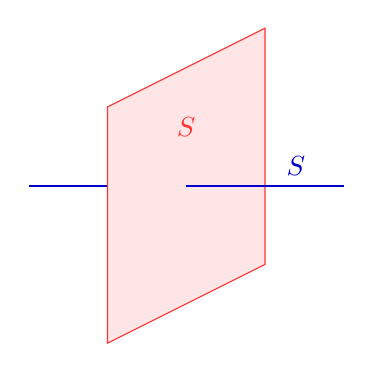
\begin{tikzpicture}[x={(1cm,0cm)},y={(1cm,0.5cm)},z={(0cm,1cm)},rotate=0]
    \draw[thick,blue!80!black](-2,0,0) -- (2,0,0);
    \filldraw[draw=red!80,fill=red!10](0,-1,-1.5) -- (0,-1,1.5) --
    (0,1,1.5) -- (0,1,-1.5) -- cycle;
    \path[red!80] (0,0,0.5) node[above] {$S$};
    \draw[thick,blue!80!black](0,0,0) -- node[above, pos=0.7] {$S^{\orth}$} (2,0,0);
  \end{tikzpicture}
\end{center}

\begin{example}{Orthogonal complement}{inner-product-orthogonal-complement}
  Consider the inner product space $\Poly_3$ of polynomials of degree
  at most $3$, with the inner product defined by
  \begin{equation*}
    \iprod{f,g} = \int_{-1}^{1} f(x)g(x)\,dx.
  \end{equation*}
  Find the orthogonal complement of $\set{x^2}$.
\end{example}

\begin{solution}
  We have to compute the set of all polynomials of the form
  $p(x)=ax^3+bx^2+cx+d$ that are orthogonal to $x^2$. So let us
  compute the inner product:
  \begin{eqnarray*}
    \iprod{p(x), x^2}
    &=& \int_{-1}^{1} (ax^3+bx^2+cx+d)x^2\,dx \\
    &=& \int_{-1}^{1} ax^5+bx^4+cx^3+dx^2\,dx \\
    &=& 0a  + \frac{2}{5}b + 0c + \frac{2}{3}d.
  \end{eqnarray*}
  Setting this equal to $0$, we see that $\iprod{p(x), x^2}=0$ if and
  only if $\frac{2}{5}b + \frac{2}{3}d = 0$, or equivalently,
  $3b+5d=0$. The basic solutions are
  \begin{equation*}
    \begin{mymatrix}{c} a \\ b \\ c \\ d \end{mymatrix}
    = \begin{mymatrix}{c} 1 \\ 0 \\ 0 \\ 0 \end{mymatrix},\quad
    \begin{mymatrix}{c} a \\ b \\ c \\ d \end{mymatrix}
    = \begin{mymatrix}{c} 0 \\ 5 \\ 0 \\ -3 \end{mymatrix},\quad
    \begin{mymatrix}{c} a \\ b \\ c \\ d \end{mymatrix}
    = \begin{mymatrix}{c} 0 \\ 0 \\ 1 \\ 0 \end{mymatrix},
  \end{equation*}
  giving the following basis for the space of polynomials orthogonal
  to $x^2$:
  \begin{equation*}
    \set{x^3,\quad 5x^2-3, \quad x}.
  \end{equation*}
\end{solution}

We now consider orthogonal sets and bases.

\begin{definition}{Orthogonal and orthonormal sets of vectors}{orthogonal-set}
  A set of vectors $\set{\vect{u}_1,\ldots,\vect{u}_k}$ in an inner
  product space is called an \textbf{orthogonal set}%
  \index{orthogonal set} if the vectors are non-zero and pairwise
  orthogonal, i.e., for all $i$, $\vect{u}_i\neq\vect{0}$ and for all
  $i\neq j$, $\vect{u}_i\orth\vect{u}_j$.
  \smallskip\smallskip

  Moreover, the set of vectors $\set{\vect{u}_1,\ldots,\vect{u}_k}$ is
  called \textbf{orthonormal}%
  \index{orthonormal set} if it is orthogonal and each vector is
  normalized, i.e., $\norm{\vect{u}_i}=1$.
\end{definition}

The interest of orthogonal and orthonormal sets of vectors lies, among
other things, in the fact that they are automatically linearly
independent.

\begin{proposition}{Orthogonal set is linearly independent}{orthogonal-linear-independence}
  If $\set{\vect{u}_1,\ldots,\vect{u}_k}$ is an orthogonal set of
  vectors, then $\vect{u}_1,\ldots,\vect{u}_k$ are linearly
  independent.
\end{proposition}

\begin{proof}
  Assume $\set{\vect{u}_1,\ldots,\vect{u}_k}$ is an orthogonal set. To
  show that $\vect{u}_1,\ldots,\vect{u}_k$ are linearly
  independent, assume
  \begin{equation*}
    a_1\vect{u}_1 + \ldots + a_k\vect{u}_k = \vect{0}.
  \end{equation*}
  We must show that $a_1,\ldots,a_k = 0$. So pick some
  $i\in\set{1,\ldots,k}$. We compute
  \begin{eqnarray*}
    \iprod{a_1\vect{u}_1 + \ldots + a_k\vect{u}_k, \vect{u}_i}
    &=& a_1\iprod{\vect{u}_1,\vect{u}_i}
        + \ldots
        + a_i\iprod{\vect{u}_i,\vect{u}_i}
        + \ldots
        + a_k\iprod{\vect{u}_k,\vect{u}_i} \\
    &=& 0
        + \ldots
        + a_i\iprod{\vect{u}_i,\vect{u}_i}
        + \ldots
        + 0 \\
    &=& a_i \iprod{\vect{u}_i,\vect{u}_i}.
  \end{eqnarray*}
  On the other hand,
  \begin{equation*}
    \iprod{a_1\vect{u}_1 + \ldots + a_k\vect{u}_k, \vect{u}_i}
    = \iprod{\vect{0}, \vect{u}_i} = 0.
  \end{equation*}
  It follows that $a_i \iprod{\vect{u}_i,\vect{u}_i} = 0$. Since
  $\iprod{\vect{u}_i,\vect{u}_i}\neq 0$, it follows that
  $a_i=0$. Since the choice of $i$ was arbitrary, it follows that
  $a_1,\ldots,a_k = 0$, and $\vect{u}_1,\ldots,\vect{u}_k$ are
  linearly independent.
\end{proof}

\begin{example}{An orthogonal set of functions}{orthogonal-set-sin-cos}
  Consider the inner product space $C[0,2\pi]$. The following
  functions form an (infinite) orthogonal set:
  \begin{eqnarray*}
    g_0(x) &=& 1 \\
    f_1(x) &=& \sin x \\
    g_1(x) &=& \cos x \\
    f_2(x) &=& \sin 2x \\
    g_2(x) &=& \cos 2x \\
    &\vdots& \\
    f_k(x) &=& \sin kx \\
    g_k(x) &=& \cos kx \\
    &\vdots&
  \end{eqnarray*}
\end{example}

\begin{proof}
  We have to check that any two functions are orthogonal to each
  other. This is true because of trigonometric identities. We have the
  following trigonometric formulas:
  \begin{eqnarray*}
    \sin\alpha\sin\beta &=& \frac{1}{2}(\cos(\alpha-\beta) - \cos(\alpha+\beta)), \\
    \cos\alpha\cos\beta &=& \frac{1}{2}(\cos(\alpha-\beta) + \cos(\alpha+\beta)), \\
    \sin\alpha\cos\beta &=& \frac{1}{2}(\sin(\alpha-\beta) + \sin(\alpha+\beta)).
  \end{eqnarray*}
  Using these, we can compute the relevant inner products. Assume $i\neq j$. Then
  \begin{eqnarray*}
    \iprod{g_i,g_j}
    &=& \int_{0}^{2\pi} \cos(ix)\cos(jx)\,dx \\
    &=& \frac{1}{2}\int_{0}^{2\pi} \cos((i-j)x) + \cos((i+j)x)\,dx \\
    &=& \frac{1}{2}\bigbracket{\frac{1}{(i-j)} \sin((i-j)x) + \frac{1}{(i+j)}
      \sin((i+j)x)}_{0}^{2\pi} \\
    &=& 0,
  \end{eqnarray*}
  and therefore $g_i\orth g_j$. The proofs of $f_i\orth f_j$ and
  $f_i\orth g_j$ are similar.
\end{proof}

\begin{definition}{Orthogonal and orthonormal bases}{orthogonal-basis}
  Let $V$ be an inner product space, and let $W$ be a subspace of
  $V$. We say that $\set{\vect{u}_1,\ldots,\vect{u}_k}$ is an
  \textbf{orthogonal basis}%
  \index{orthogonal basis}%
  \index{basis!orthogonal} for $W$ if it is an orthogonal set and
  spans $W$.
  \smallskip\smallskip

  If, moreover, each $\vect{u}_i$ is normalized, we say that
  $\set{\vect{u}_1,\ldots,\vect{u}_k}$ is an \textbf{orthonormal
    basis}%
  \index{orthonormal basis}%
  \index{basis!orthonormal} for $W$.
\end{definition}

We note that, by
Proposition~\ref{prop:orthogonal-linear-independence}, every
orthogonal (or orthonormal) basis is automatically linearly
independent, and therefore an actual basis of $W$.

\begin{example}{Orthogonal, orthonormal, and non-orthogonal bases}{orthogonal-basis}
  Consider $\R^2$ as an inner product space with the usual dot product.
  \begin{itemize}
  \item $\set{\begin{mymatrix}{r} 1 \\ 0 \end{mymatrix},
      \begin{mymatrix}{r} 0 \\ 1 \end{mymatrix}}$ is an orthonormal
    basis of $\R^2$.
  \item
    $\set{\frac{1}{\sqrt{2}}\begin{mymatrix}{r} 1 \\ 1 \end{mymatrix},
      \frac{1}{\sqrt{2}}\begin{mymatrix}{r} 1 \\ -1 \end{mymatrix}}$
    is an orthonormal basis of $\R^2$.
  \item $\set{\begin{mymatrix}{r} 2 \\ 0 \end{mymatrix},
      \begin{mymatrix}{r} 0 \\ 3 \end{mymatrix}}$ is an orthogonal
    basis of $\R^2$, but not orthonormal.
  \item $\set{\begin{mymatrix}{r} 1 \\ 1 \end{mymatrix},
      \begin{mymatrix}{r} 1 \\ -1 \end{mymatrix}}$ is an orthogonal
    basis of $\R^2$, but not orthonormal.
  \item $\set{\begin{mymatrix}{r} 1 \\ 0 \end{mymatrix},
      \begin{mymatrix}{r} 1 \\ 1 \end{mymatrix}}$ is a basis of
    $\R^2$, but neither orthogonal nor orthonormal.
  \end{itemize}
\end{example}

So why are we interested in orthogonal and orthonormal bases? The main
reason is that finding coordinates is {\em much easier} when the bases
are orthogonal (and even better when they are orthonormal). We have
the following property:

\begin{proposition}{Fourier coefficients}{fourier-coefficients}
  Let $B=\set{\vect{u}_1,\ldots,\vect{u}_n}$ be an orthogonal basis of
  some space $W$, and suppose $\vect{v}\in W$. Then
  \begin{equation*}
    \vect{v} = a_1\vect{u}_1 + \ldots + a_n\vect{u}_n,
  \end{equation*}
  where
  \begin{equation*}
    a_i = \frac{\iprod{\vect{u}_i,\vect{v}}}{\iprod{\vect{u}_i,\vect{u}_i}}.
  \end{equation*}
  In this situation, the coordinates $a_1,\ldots,a_n$ are also called
  the \textbf{Fourier coefficients}%
  \index{Fourier coefficients} of $\vect{v}$ (with respect to the
  orthogonal basis $B$).
  \smallskip\smallskip

  In case $B$ is an orthonormal basis, the formula is even simpler. In
  that case:
    \begin{equation*}
    a_i = \iprod{\vect{u}_i,\vect{v}}.
  \end{equation*}
\end{proposition}

\begin{proof}
  Since $B$ is a basis of $W$, we know that there exist coefficients
  $a_1,\ldots,a_n$ such that
  $\vect{v} = a_1\vect{u}_1 + \ldots + a_n\vect{u}_n$. It remains to
  verify that the coefficients satisfy the required formula. This is a
  simple calculation. We have
  \begin{eqnarray*}
    \iprod{\vect{u}_i,\vect{v}}
    &=& \iprod{\vect{u}_i, a_1\vect{u}_1 + \ldots + a_n\vect{u}_n} \\
    &=& a_1\iprod{\vect{u}_i,\vect{u}_1}
        + \ldots
        + a_i\iprod{\vect{u}_i,\vect{u}_i}
        + \ldots
        + a_n\iprod{\vect{u}_i,\vect{u}_n} \\
    &=& 0
        + \ldots
        + a_i\iprod{\vect{u}_i,\vect{u}_i}
        + \ldots
        + 0 \\
    &=& a_i \iprod{\vect{u}_i,\vect{u}_i}.
  \end{eqnarray*}
  Since $\vect{u}_i\neq \vect{0}$, we have
  $\iprod{\vect{u}_i,\vect{u}_i}\neq 0$ by the positive definite
  property. We can therefore divide both sides of the equation by
  $\iprod{\vect{u}_i,\vect{u}_i}$ to obtain
  \begin{equation*}
    a_i = \frac{\iprod{\vect{u}_i,\vect{v}}}{\iprod{\vect{u}_i,\vect{u}_i}},
  \end{equation*}
  as desired. Finally, if the basis is orthonormal, then
  $\iprod{\vect{u}_i,\vect{u}_i}=1$, and the denominator disappears,
  so that $a_i = \iprod{\vect{u}_i,\vect{v}}$.
\end{proof}

\begin{example}{Fourier coefficients}{fourier-coefficients}
  Suppose $B=\set{\vect{u}_1,\vect{u}_2,\vect{u}_3}$ is an orthogonal
  basis for an inner product space $V$, such that
  $\norm{\vect{u}_1}=1$, $\norm{\vect{u}_2}=\sqrt{2}$, and
  $\norm{\vect{u}_3}=2$.  Moreover, suppose that $\vect{v}\in V$ is a
  vector such that $\iprod{\vect{v},\vect{u}_1} = 3$,
  $\iprod{\vect{v},\vect{u}_2} = -1$, and
  $\iprod{\vect{v},\vect{u}_3} = 2$.  Find the coordinates of
  $\vect{v}$ with respect to $B$.
\end{example}

\begin{solution}
  We have to find $a_1,a_2,a_3$ such that
  \begin{equation*}
    \vect{v} = a_1\vect{u}_1 + a_2\vect{u}_2 + a_3\vect{u}_3.
  \end{equation*}
  We have sufficient information to compute $a_1,a_2,a_3$. Namely,
  \begin{eqnarray*}
    a_1
    &=& \frac{\iprod{\vect{u}_1,\vect{v}}}{\iprod{\vect{u}_1,\vect{u}_1}}
        ~=~ \frac{\iprod{\vect{u}_1,\vect{v}}}{\norm{\vect{u}_1}^2}
        ~=~ \frac{3}{1} ~=~ 3, \\
    a_2
    &=& \frac{\iprod{\vect{u}_2,\vect{v}}}{\iprod{\vect{u}_2,\vect{u}_2}}
        ~=~ \frac{\iprod{\vect{u}_2,\vect{v}}}{\norm{\vect{u}_2}^2}
        ~=~ \frac{-1}{2} ~=~ -0.5, \\
    a_3
    &=& \frac{\iprod{\vect{u}_3,\vect{v}}}{\iprod{\vect{u}_3,\vect{u}_3}}
        ~=~ \frac{\iprod{\vect{u}_3,\vect{v}}}{\norm{\vect{u}_3}^2}
        ~=~ \frac{2}{4} ~=~ 0.5.
  \end{eqnarray*}
\end{solution}

Proposition~\ref{prop:fourier-coefficients} shows that if
$\set{\vect{u}_1,\ldots,\vect{u}_n}$ is an orthogonal basis, then we
can solve $\vect{v} = a_1\vect{u}_1 + \ldots + a_n\vect{u}_n$ without
having to solve a system of equations. While this is a useful thing to
be able to do, perhaps it is merely a convenience (solving a system of
equations would also be fine). However, there is another very useful
property of Fourier coefficients. The coefficient $a_i$ only depends
on the basis vector $\vect{u}_i$, and not on any of the other basis
vectors. This is useful in situations where only {\em part} of an
orthogonal basis is known. We can calculate the corresponding
coefficients without having to know the rest of the basis.

\begin{example}{Finding partial coordinates}{partial-coordinates}
  Suppose $B=\set{\vect{u}_1,\vect{u}_2,\vect{u}_3,\vect{u}_4}$ is an
  orthogonal basis of $\R^4$. We have been told that
  \begin{equation*}
    \vect{u}_1 = \begin{mymatrix}{c} 1 \\ 2 \\ -1 \\ 0 \end{mymatrix}
    \quad\mbox{and}\quad
    \vect{u}_2 = \begin{mymatrix}{c} 0 \\ 1 \\ 2 \\ 3 \end{mymatrix},
  \end{equation*}
  but it is not known what $\vect{u}_3$ and $\vect{u}_4$ are. Find the
  first two coordinates of the vector
  \begin{equation*}
    \vect{v} = \begin{mymatrix}{c} 1 \\ 0 \\ 2 \\ 0 \end{mymatrix}
  \end{equation*}
  with respect to the basis $B$.
\end{example}

\begin{solution}
  We have $\vect{v} = a_1\vect{u}_1 + a_2\vect{u}_2 + a_3\vect{u}_3 +
  a_4\vect{u}_4$, where
  \begin{equation*}
    a_1
    = \frac{\iprod{\vect{u}_1,\vect{v}}}{\iprod{\vect{u}_1,\vect{u}_1}}
    = \frac{-1}{6}
    \quad\mbox{and}\quad
    a_2
    = \frac{\iprod{\vect{u}_2,\vect{v}}}{\iprod{\vect{u}_2,\vect{u}_2}}
    = \frac{4}{14}.
  \end{equation*}
  So the first two coordinates are $-\frac{1}{6}$ and $\frac{2}{7}$.
\end{solution}

A word of warning is in order: Fourier coefficients do not work when
the basis is not orthogonal. Consider the following picture, where
$\vect{u}_1$ and $\vect{u}_2$ are not orthogonal.
\begin{equation*}
  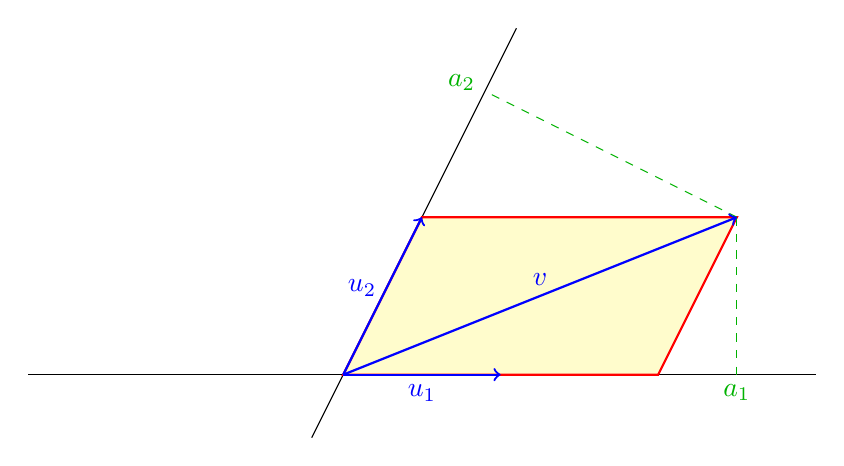
\begin{tikzpicture}[scale=2]
    \draw (-2,0) -- (3,0);
    \draw (-0.2,-0.4) -- (1.1,2.2);
    \draw[thick,red,fill=yellow!20] (0,0) -- (2,0) -- (2.5,1) -- (0.5,1) -- cycle;
    \draw[dashed,green!70!black] (2.5,1) -- (2.5,0) node[below]{$a_1$};
    \draw[dashed,green!70!black] (2.5,1) -- (0.9,1.8) node[left,yshift=3]{$a_2$};
    \draw[thick,blue,->] (0,0) -- node[below]{$\vect{u}_1$} (1,0);
    \draw[thick,blue,->] (0,0) -- node[left, pos=0.55]{$\vect{u}_2$} (0.5,1);
    \draw[thick,blue,->] (0,0) -- node[above]{$\vect{v}$} (2.5,1);
  \end{tikzpicture}
\end{equation*}
The {\em coordinates} of $\vect{v}$ with respect to
$\vect{u}_1,\vect{u}_2$ are $(2,1)$, because
$\vect{v}=2\vect{u}_1+1\vect{u}_2$, as indicated by the shaded
parallelogram. On the other hand, the formula for the {\em Fourier
  coefficients} is concerned with the orthogonal projections of
$\vect{v}$ onto $\vect{u}_1$ and $\vect{u}_2$, as indicated by the
dashed lines. It yields the coefficients
\begin{eqnarray*}
  a_1 &=& \frac{\iprod{\vect{u}_1,\vect{v}}}{\iprod{\vect{u}_1,\vect{u}_1}} ~\approx~ 2.5, \\
  a_2 &=& \frac{\iprod{\vect{u}_2,\vect{v}}}{\iprod{\vect{u}_2,\vect{u}_2}} ~\approx~ 1.8. \\
\end{eqnarray*}
These are not the same as the coordinates of $\vect{v}$, because the
dashed lines are orthogonal to $\vect{u}_1$ and $\vect{u}_2$, instead
of parallel to them. In summary, the Fourier coefficients of a vector
are equal to its coordinates {\em only if the basis is orthogonal}.

We conclude this section by making a connection between arbitrary
inner products and dot products.  Once an orthonormal basis has been
chosen on an inner product space, computing inner products is
essentially the same as computing dot products. The following
proposition makes this more precise.

\begin{proposition}{Inner product and dot product}{inner-product-dot-product}
  Let $V$ be an inner product space, and suppose that
  $B=\set{\vect{u}_1,\ldots\vect{u}_n}$ is an orthonormal basis. Then
  for any pair of vectors $\vect{v},\vect{w}\in V$, their inner
  product is equal to the dot product of their coordinate vectors with
  respect to the basis $B$, i.e.
  \begin{equation*}
    \iprod{\vect{v},\vect{w}}
    = \coord{\vect{v}}_B \dotprod \coord{\vect{w}}_B.
  \end{equation*}
\end{proposition}

\begin{proof}
  By definition of coordinate vectors, we have
  \begin{equation*}
    \coord{\vect{v}}_B
    = \begin{mymatrix}{c} a_1 \\ \vdots \\ a_n \end{mymatrix}
    \quad\mbox{and}\quad
    \coord{\vect{w}}_B
    = \begin{mymatrix}{c} b_1 \\ \vdots \\ b_n \end{mymatrix},
  \end{equation*}    
  where $\vect{v} = a_1\vect{u}_1 + \ldots + a_n\vect{u}_n$ 
  and $\vect{w} = b_1\vect{u}_1 + \ldots + b_n\vect{u}_n$.
  We calculate
  \begin{eqnarray*}
    \iprod{\vect{v},\vect{w}}
    &=& \iprod{a_1\vect{u}_1 + \ldots + a_n\vect{u}_n, b_1\vect{u}_1 +
        \ldots + b_n\vect{u}_n} \\
    &=& \begin{array}[t]{@{}c@{~}c@{~}c@{~}c@{~}c@{~}c@{~}c@{~}c}
          &   a_1b_1\iprod{\vect{u}_1,\vect{u}_1}
          &+& a_1b_2\iprod{\vect{u}_1,\vect{u}_2}
          &+& \ldots
          &+& a_1b_n\iprod{\vect{u}_1,\vect{u}_n} \\
          +&  a_2b_1\iprod{\vect{u}_2,\vect{u}_1} 
          &+& a_2b_2\iprod{\vect{u}_2,\vect{u}_2}
          &+& \ldots
          &+& a_2b_n\iprod{\vect{u}_2,\vect{u}_n} \\
          +&  \vdots
          && \vdots
          && 
          && \vdots \\
          +&  a_nb_1\iprod{\vect{u}_n,\vect{u}_1}
          &+& a_nb_2\iprod{\vect{u}_n,\vect{u}_2}
          &+& \ldots
          &+& a_nb_n\iprod{\vect{u}_n,\vect{u}_n}
        \end{array} \\
    &=& a_1b_1 + a_2b_2 + \ldots + a_nb_n \\
    &=& \coord{\vect{v}}_B \dotprod \coord{\vect{w}}_B.        
  \end{eqnarray*}
  Here we have used the fact that $\iprod{\vect{u}_i,\vect{u}_j}=1$
  when $i=j$ and $\iprod{\vect{u}_i,\vect{u}_j}=0$ otherwise, which
  holds because $B$ is orthonormal.
\end{proof}
